\chapter{Heap}


\section{Introduction}
Heap-ordered. Binary heap is one of the implementations of Priority Queue (ADT). 

Basic options:
\begin{enumerate}
\item sink()/ sift\_down() - recursive
\item swim()/ sift\_up() - recursive
\item build()/ heapify() - bottom-up sink()
\end{enumerate}
\section{Implementation}
The self-implemented binary heap's index usually starts at 1 rather than 0. 
\begin{figure}[hbtp]
\centering
\subfloat{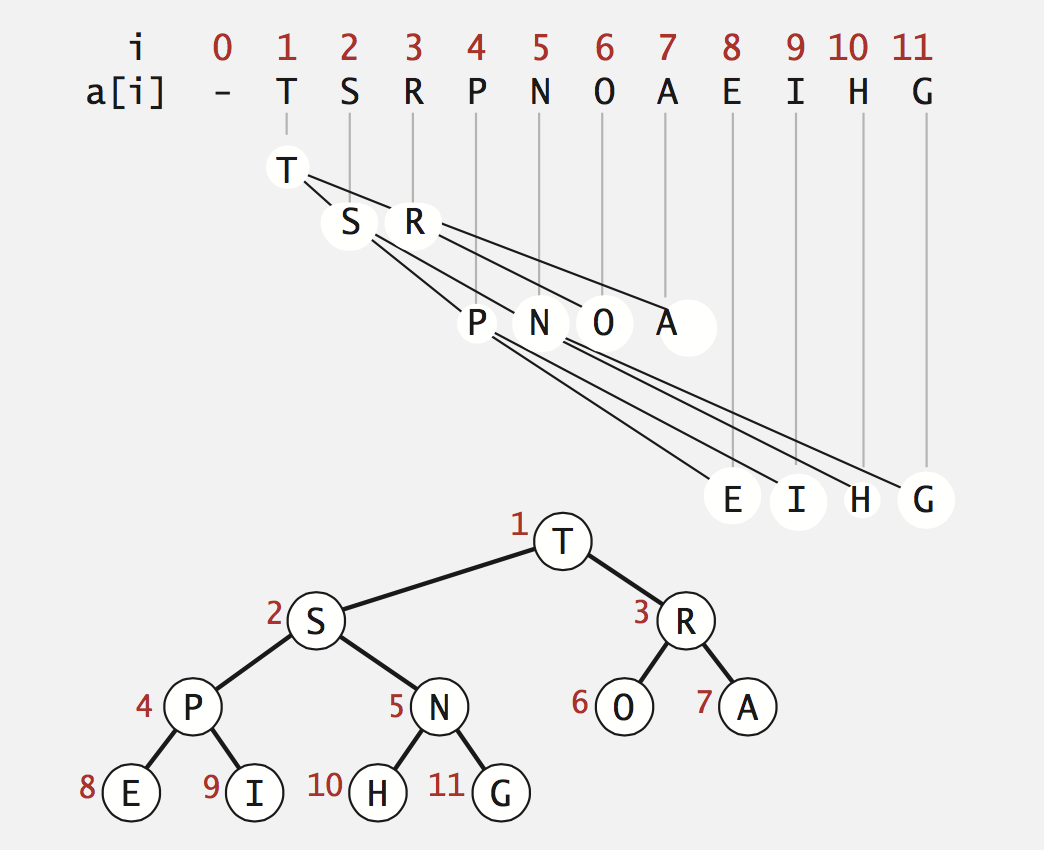
\includegraphics[scale=.80]{heap_repr}}
\caption{Heap representation}
\label{fig:heap} 
\end{figure}

\section{Python heapq}
Python only has built in min-heap. To use max-heap, you can: 
\begin{enumerate}
\item Revert the number: 1 becomes -1.
\item Wrap the data into another class and override \textbf{comparators}: \_\_cmp\_\_ or \_\_lt\_\_
\end{enumerate}

The following code presents the wrapping method:
\begin{python}
class Value(object):
    def __init__(self, val):
        self.val = val
        self.deleted = False  # lazy delete 

    def __cmp__(self, other):
        # Reverse order by height to get max-heap
        assert isinstance(other, Value)
        return other.val - self.val
\end{python}

Normally the deletion by value in Python is $O(n)$, to achieve $O(\lg n)$ we can use \textbf{lazy deletion}. Before take the top of the heap, we do the following:
\begin{python}
while heap and heap[0].deleted:
    heapq.heappop(heap)
\end{python}
\subsection{Complexity}
Building a heap is O(N) rather than $O(N \lg N)$.

Proof:
\begin{eqnarray*}
&& \because \sum_{i=0}^{+\infty} {ix^i} =\frac{x}{(1-x)^2} \\
&& \therefore \sum_{h=0}^{\lfloor\lg n\rfloor}{\Big\lceil\frac{n}{2^{h+1}}\Big\rceil O(h)} = O\Bigg(n\sum_{h=0}^{\lfloor\lg n\rfloor}{\frac{h}{2^h}}\Bigg) \\
&& \therefore \sum_{h=0}^{\lfloor\lg n\rfloor}{\Big\lceil\frac{n}{2^{h+1}}\Big\rceil
O(h)} = O(n)
\end{eqnarray*}
